\tolerance=10000
\documentclass[conference]{IEEEtran}
\usepackage{xcolor}
\usepackage{mathtools}
\usepackage{enumerate}
\usepackage{hyperref}
\usepackage{amssymb}
\usepackage{amsmath}
\usepackage{eqnarray}
\usepackage[]{algorithm}
\usepackage{clrscode3e}
\usepackage[pdftex]{graphicx}

%\usepackage{etoolbox}
%\AtBeginEnvironment{algorithmic}{\small}
%\usepackage{subfig}
% tricks for saving space
\usepackage[font={small}]{caption,subfig}  % small fonts in captions
\setlength{\abovecaptionskip}{1ex}
\setlength{\belowcaptionskip}{1ex}
\setlength{\floatsep}{1ex}
\setlength{\textfloatsep}{1ex}

\DeclarePairedDelimiter{\ceil}{\lceil}{\rceil}
\DeclarePairedDelimiter{\floor}{\lfloor}{\rfloor}

\begin{document}

%%%%%%%%%%%%%%%%%%%%%%%%%%%%%%%%%%%%%%%%%%%%%%%%%%%%%%%%%%%%%%%%%%%%%%%
%%%%%%%%%%%%%%%%%%%%%%%%%%%%%%%%%%%%%%%%%%%%%%%%%%%%%%%%%%%%%%%%%%%%%%%
%%
%% TITLE
%%
%%%%%%%%%%%%%%%%%%%%%%%%%%%%%%%%%%%%%%%%%%%%%%%%%%%%%%%%%%%%%%%%%%%%%%%
%%%%%%%%%%%%%%%%%%%%%%%%%%%%%%%%%%%%%%%%%%%%%%%%%%%%%%%%%%%%%%%%%%%%%%%

\title{ZNN\emph{i} -- Maximizing the Inference Throughput of 3D
  Convolutional Networks on Multi-Core Machines and GPUs}

\author{\IEEEauthorblockN{Aleksandar Zlateski\IEEEauthorrefmark{1},
    Kisuk Lee\IEEEauthorrefmark{2}}
  \IEEEauthorblockA{\IEEEauthorrefmark{1}Electrical Engineering and
    Computer Science Dept.\\ \IEEEauthorrefmark{2}Brain and
    Cognitive Sciences Dept.\\ Massachusetts Institute of
    Technology\\ Cambridge, MA 02139 USA\\ \IEEEauthorrefmark{1}{\tt
      zlateski@mit.edu}, \IEEEauthorrefmark{2}{\tt kisuklee@mit.edu}}
  \and \IEEEauthorblockN{H. Sebastian Seung}
  \IEEEauthorblockA{Princeton Neuroscience Institute\\ and Computer
    Science Dept.\\ Princeton University\\ Princeton, NJ 08540
    USA\\ {\tt sseung@princeton.edu} }}


\maketitle
%\thispagestyle{empty}

%%%%%%%%%%%%%%%%%%%%%%%%%%%%%%%%%%%%%%%%%%%%%%%%%%%%%%%%%%%%%%%%%%%%%%%
%%%%%%%%%%%%%%%%%%%%%%%%%%%%%%%%%%%%%%%%%%%%%%%%%%%%%%%%%%%%%%%%%%%%%%%
%%
%% ABSTRACT
%%
%%%%%%%%%%%%%%%%%%%%%%%%%%%%%%%%%%%%%%%%%%%%%%%%%%%%%%%%%%%%%%%%%%%%%%%
%%%%%%%%%%%%%%%%%%%%%%%%%%%%%%%%%%%%%%%%%%%%%%%%%%%%%%%%%%%%%%%%%%%%%%%


\begin{abstract}

We present a novel parallel algorithm for 3D ConvNet inference on
multi-core shared memory machines.  We also present a novel algorithm
for ConvNet inference on the GPU that uses less memory.  We also
present an algorithm that uses the GPU and host ram to improve the
throughput.  As well as CPU-GPU combined algorithm.

We compare discuss the advantages and disadvantages of all approaches.

We compare our algorithms to publicly available implementation (on the
same hardware) and observe great speedup.

\end{abstract}

%%%%%%%%%%%%%%%%%%%%%%%%%%%%%%%%%%%%%%%%%%%%%%%%%%%%%%%%%%%%%%%%%%%%%%%
%%%%%%%%%%%%%%%%%%%%%%%%%%%%%%%%%%%%%%%%%%%%%%%%%%%%%%%%%%%%%%%%%%%%%%%
%%
%% INTRODUCTION
%%
%%%%%%%%%%%%%%%%%%%%%%%%%%%%%%%%%%%%%%%%%%%%%%%%%%%%%%%%%%%%%%%%%%%%%%%
%%%%%%%%%%%%%%%%%%%%%%%%%%%%%%%%%%%%%%%%%%%%%%%%%%%%%%%%%%%%%%%%%%%%%%%

\section{Introduction}

cuDNN is described here~\cite{chetlur2014cudnn}

We do max fragment pooling as described here~\cite{giusti2013fast}.
Except that we are limiting the sizes of our output patches to have
each dimension equal to the cartesian product of all corresponding
dimensions of all pooling windows in the network.

We care about throughput -- not latency in this case.  This is because
we assume that we need to do inference on a large amount of data.

Hence, self-tuning time and latency are negligible.  Self-tuning
because it only has to be done once; latency because the data is huge.
Examples -- videos, EM data, tons of images (FB?).

Relate to ZNN for training as training has to be optimized for
latency.

\section{Max fragment pooling}

We should not use batches (except sometimes)

\begin{figure}
  \centering
  \subfloat[]{\protect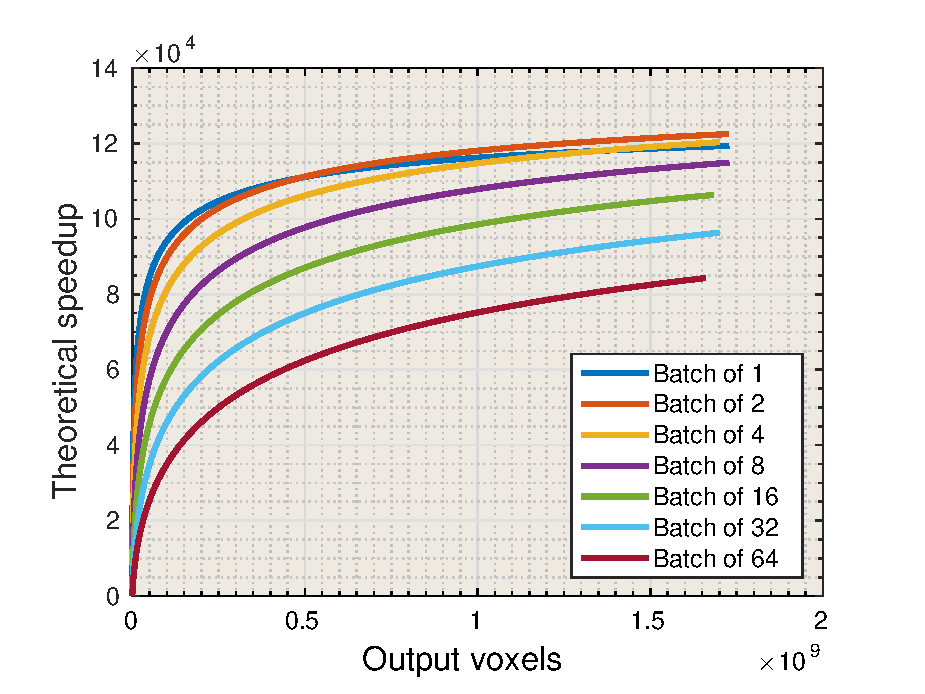
\includegraphics[width=0.24\textwidth]
    {fig/fft_batch_speedup.eps}}
  \subfloat[]{\protect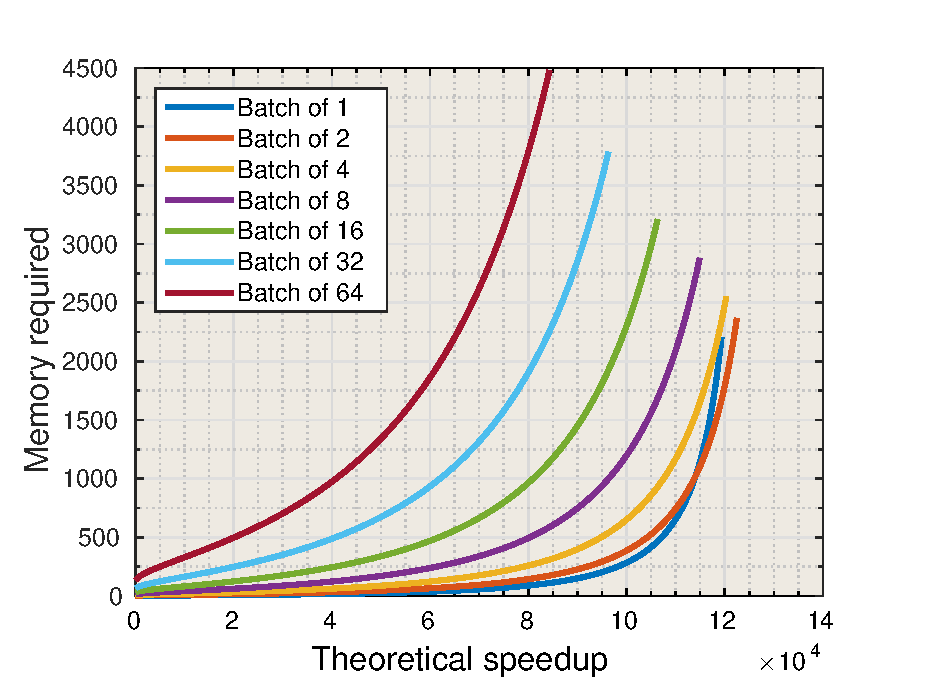
\includegraphics[width=0.24\textwidth]
    {fig/fft_mem_speedup.eps}}

  \caption{Explains why we should not use batches ever!}
  \label{fig:batch_explanation}
\end{figure}



We reduce the number of operations per output sample by:
\begin{enumerate}
\item Using sliding window inference by kernel rarefication.
\item Choosing optimal size for the output image as well as the batch
  size.
\item Using \emph{pruned FFTs} for computing the FFTs of the kernels.
\end{enumerate}

We improve the throughput by parallelizing the algorithm over multiple
available cores, while using little memory overhead per running
thread.


\section{Padded pruned FFT}

A 3D FFT transform is obtained by computing 1D FFTs along the three
dimensions.  When computing a transform of a padded 3D image, many of
these 1D transforms will operate on all $0$ elements.  These
transforms are unnecessary as FFT of a zero vector is a zero vector.

A convolution of a 3D image with a kernel is obtained by first zero
padding the image and the kernel to the same size, after which we
perform the transform of both the padded image and kernel.  The
inverse transform of the point-wise product of the two transforms will
contain the result of the convolution.

We can reduce the amount of computation by computing only necessary 1D
transforms.  For instance, when computing the FFT of trainable kernel
of size $k^3$ zero padded to size of $n^3$, instead of naively
computing $n^2$ 1D FFTs each dimension, which takes $C n^3 \log n^3$
we could first only do $k^2$ FFTs along one direction, then $k \times
x$ along then next, and finally $n^2$ along the last direction.  This
way we reduce the computational cost from $C n^3 \log n^3$ to $C n\log
n[k^2 + k \cdot n + n^2]$.  As most of the FFTs are performed on
kernels, when $k << n$, we could reduce the computation cost by almost
two thirds.


\begin{figure}
  \begin{center}
  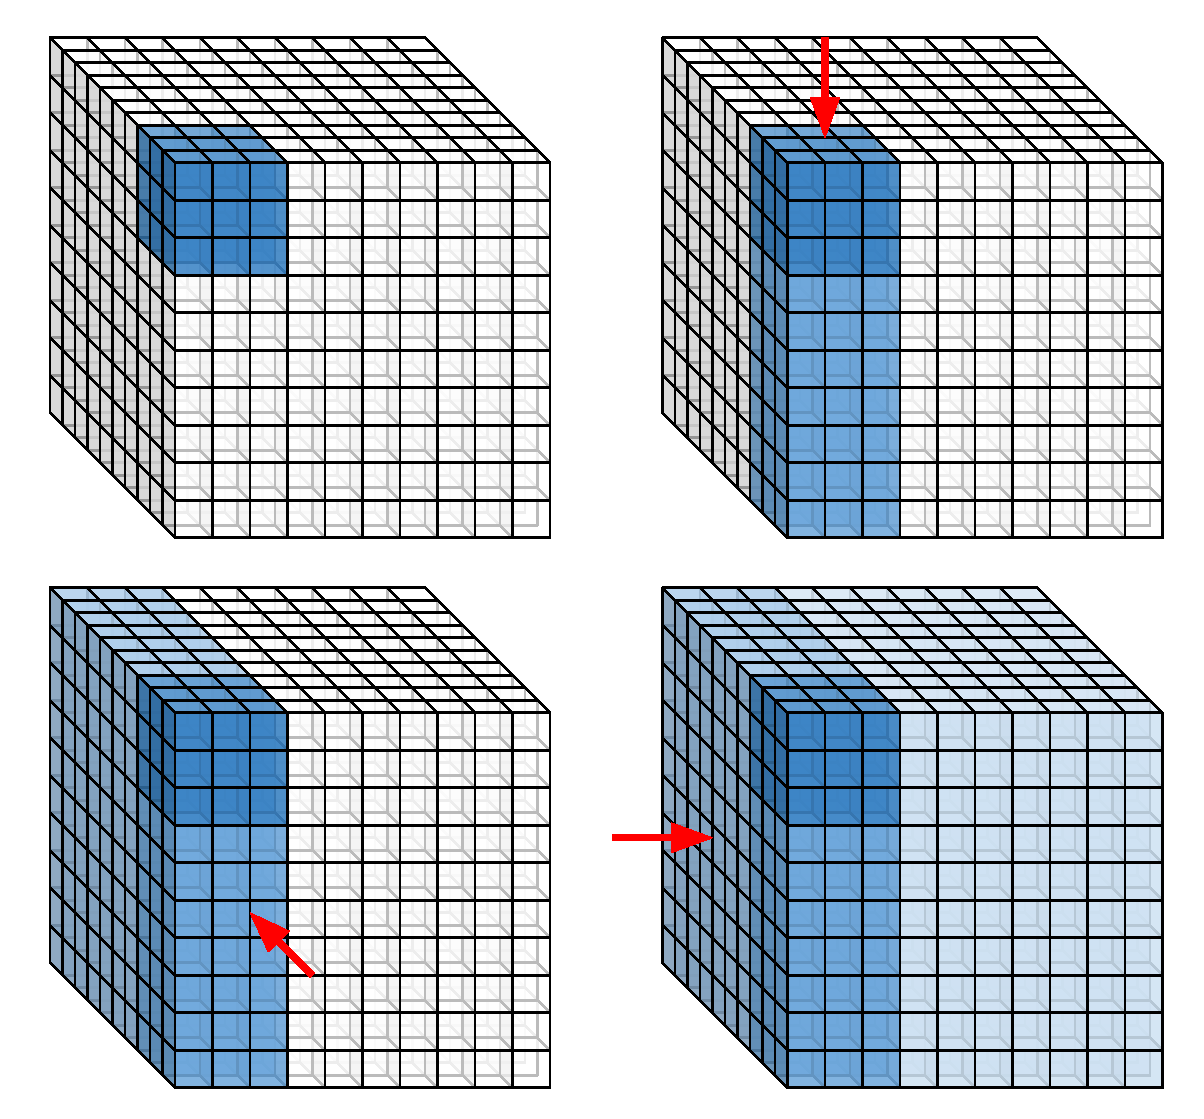
\includegraphics[width=0.65\columnwidth]{fig/pruned_ffts.pdf}
  \end{center}
  \caption{Pruned FFTs.}
  \label{fig:pruned_ffts}
\end{figure}

\subsection{CPU implementation}

We describe how the serial padded pruned FFT and iFFT is done.

We also describe how we parallelize a single FFT.

When fftw is used, we only use sizes of $2^a3^b5^c7^d11^e13^f$ where
$e+f$ is either $1$ or $0$~\cite{frigo1999fftw,frigo1998fftw}.

When using mkl fft we only use sizes of $2^a3^b5^c7^d11^e13^f$.

\subsection{GPU implementation}

On the gpu we only use sizes  $2^a3^b5^c7^d$~\cite{nvidia2010cufft}.

We always do a batch of 3D FFTs (imagine as 4D tensor)

On the gpu.  For index calculation we use~\cite{warren2013hacker}

Assume that we want to compute the FFT transforms of $b$ 3D images
each of size $x_i \times y_i \times z_i$.  We first compute the
optimal size for the transform independently in each of the three
dimensions.  Let it be $x_o \times y_o \times z_o$.  The images are
stored in a row major form in memory as a 4D row major matrix of real
numbers with the dimension of $b \times x_i \times y_i \times z_i$.

We first perform in--place real to complex 1D transforms along the $z$
direction. We prepare the input by extending the 4D matrix along the
$z$ direction to fit the result.  The transform will need to contain
$z_o' = z_o / 2 + 1$ complex numbers, and we need twice as many reals.
A matrix of size $b \times x_i \times y_i \times 2z_o')$ is first
initialized to zero, and appropriate elements from the input are
filled in.  After batched in--place real to complex 1D transforms are
performed.  The result represents a 4D matrix of complex numbers of
size $b \times x_i \times y_i \times z_o'$.  Note that all the 1D
transforms are done on contiguous memory chunks (along the least
significant dimension).

In the next step we perform in-place complex to complex transforms
along the $y$ direction.  To do that we will flip the dimensions and
zero pad the previous matrix.  First we initialize a matrix of complex
numbers with the size of $b \times x_i \times z_o' \times y_o$.  The
matrix is first initialized to zero.  Each element $i,j,k,l$ of the
input matrix is mapped to $i,j,l,k$.  Then $b \times x_i \times z_o'$
1D transforms are performed along the last dimension.

Finally we perform the last in-place complex to complex transform
along the $x$ direction.  For that we initialize $b \times z_o' \times
y_o \times x_o$ matrix to all zeros.  An element $i,j,k,l$ from the
previous result gets mapped to an element $i,k,l,j$.  Once again we
perform $b \times z_o' \times y_o$ 1D in--place transforms, once again
on contiguous chunks.

We keep this as the output shape, as we only care about being able to
perform point--wise operations on the image transform.  The backward
transform is done in a similar fashion just taking the steps in the
reverse.

4D matrix reshaping requires a lot of index to index calculation,
which can involve a lot expensive division and modulus operations.
Sometimes these operations are more expensive than the actual 1D
transforms performed.  We improve the performances by only using
multiplications by a pre--computed magic numbers and shift operations
as described in ~\cite{warren2013hacker}.  Image reshaping is easily
implemented using the Thrust CUDA library~\cite{bell2011thrust}.

\section{Algorithms for the convolutional layers}

In each algorithm we assume that we need to perform the computation of
a convolutional layer with $f$ input feature-maps and $f'$ output
feature-maps.  Each algorithm evaluates the layer on a batch of size
$b$ inputs.  Let the size of each input image be $x \times y \times
z$.  We represent the input as a 5D tensor with size $b \times
f \times x \times y \times z$, and the output as a 5D tensor with the
size $b \times f' \times x \times y \times z$.  The tensors are stored
in memory in the row major (commonly known as C) order.

\subsection{CPU algorithms}

We present two algorithms suited for multi-core CPUs.  The two
algorithms have different parallelization strategies and yield
different performance and memory usage.

Both algorithm consist of three stages.  In the first stage all the
transforms of the inputs are computed.  In the second stage FFTs of
the kernels are computed and point-wise products are accumulated.
Finally in the third stage the inverse transforms of the accumulated
products are computed obtaining the output images.

Breaking up the algorithm into three stages allows us to more
efficiently utilize the available memory.  After the first stage, the
memory used by the input images is not required, and can be freed.
After the second stage the memory used by the transforms of the input
images can also be freed.

\subsubsection{Direct convolution algorithm}

\begin{algorithm}
  {\small
  \begin{codebox}
    \Procname{$\proc{Convolutional-Forward-FFT-CPU1}(I,w,b,f,f',\vec{n},\vec{k})$}
    \li $\vec{n}' = \vec{n} - \vec{k} + \vec{1}$
    \li $O \gets \proc{5D-Real-Tensor}(b,f',n'_x,n'_y,n'_z)$
    \li \kw{Parfor} $i \gets 0 \To b-1$
    \li   \Do \kw{Parfor} $j \gets 0 \To f'-1$
    \li     \Do \For $k \gets 0 \To f-1$
    \li     \Do $O_{i,j} \gets O_{i,j} + \proc{Convolve}(I_{i,k},w_{j,k})$
    \End \End \End
    \li $\proc{Free-Memory}(I)$
    \li \Return $O$
  \end{codebox}
  }

  \caption{Multi-core algorithm for a convolutional layer using direct
  convolution.}
  \label{alg:cpu_direct}
\end{algorithm}

\subsubsection{FFT based algorithm 1}

The first algorithm is very similar to the serial algorithm and is
given in the algorithm listing~\ref{alg:cpu_alg1}.  The computationally
intensive operations in the algorithm are individually parallelized.
More specifically each FFT and inverse FFT transform is done in
parallel as explained above.  The $\proc{Parallel-MAD}$ function
computes a series of multiply-add operations in parallel by dividing
the range into roughly equal sub-ranges, each of which is executed on
a single core.

\begin{algorithm}
  {\small
  \begin{codebox}
    \Procname{$\proc{Convolutional-Forward-FFT-CPU1}(I,w,b,f,f',x,y,z)$}
    \li $\widetilde{I} \gets \proc{5D-Complex-Tensor}(b,f,\floor{x/2}+1,y,z)$
    \li \For $i \gets 0 \To b-1$
    \li   \Do \For $j \gets 0 \To f-1$
    \li     \Do $\widetilde{I}_{i,j} \gets \proc{Parallel-FFT}(I_{i,j})$
    \End \End
    \li $\proc{Free-Memory}(I)$
    \li $\widetilde{O} \gets \proc{5D-Complex-Tensor}(b,f',\floor{x/2}+1,y,z)$
    \li \For $i \gets 0 \To f'-1$
    \li   \Do \For $j \gets 0 \To f-1$
    \li     \Do $\widetilde{w}_{i,j} = \proc{Parallel-FFT}(w_{i,j})$
    \li         \For $k \gets 0 \To b-1$
    \li           \Do $\proc{Parallel-MAD}(\widetilde{O}_{k,j}, \widetilde{w}_{i,j}, \widetilde{O}_{k,i})$
    \End \End \End
    \li $\proc{Free-Memory}(\widetilde{I})$
    \li $O \gets \proc{5D-Real-Tensor}(b,f',x,y,z)$
    \li \For $i \gets 0 \To b-1$
    \li   \Do \For $j \gets 0 \To f'-1$
    \li     \Do $O_{i,j} \gets \proc{Parallel-Inverse-FFT}(\widetilde{O}_{i,j})$
    \End \End
    \li $\proc{Free-Memory}(\widetilde{O})$
    \li \Return $O$
  \end{codebox}
  }

  \caption{Multi-core algorithm for a convolutional
  layer}
  \label{alg:cpu_alg1}
\end{algorithm}

The memory requirement of the algorithm equals to the maximal amount
of memory required by the algorithm at any single point of time during
the execution.

\subsubsection{FFT based algorithm 2}

\begin{figure}
  \begin{center}
  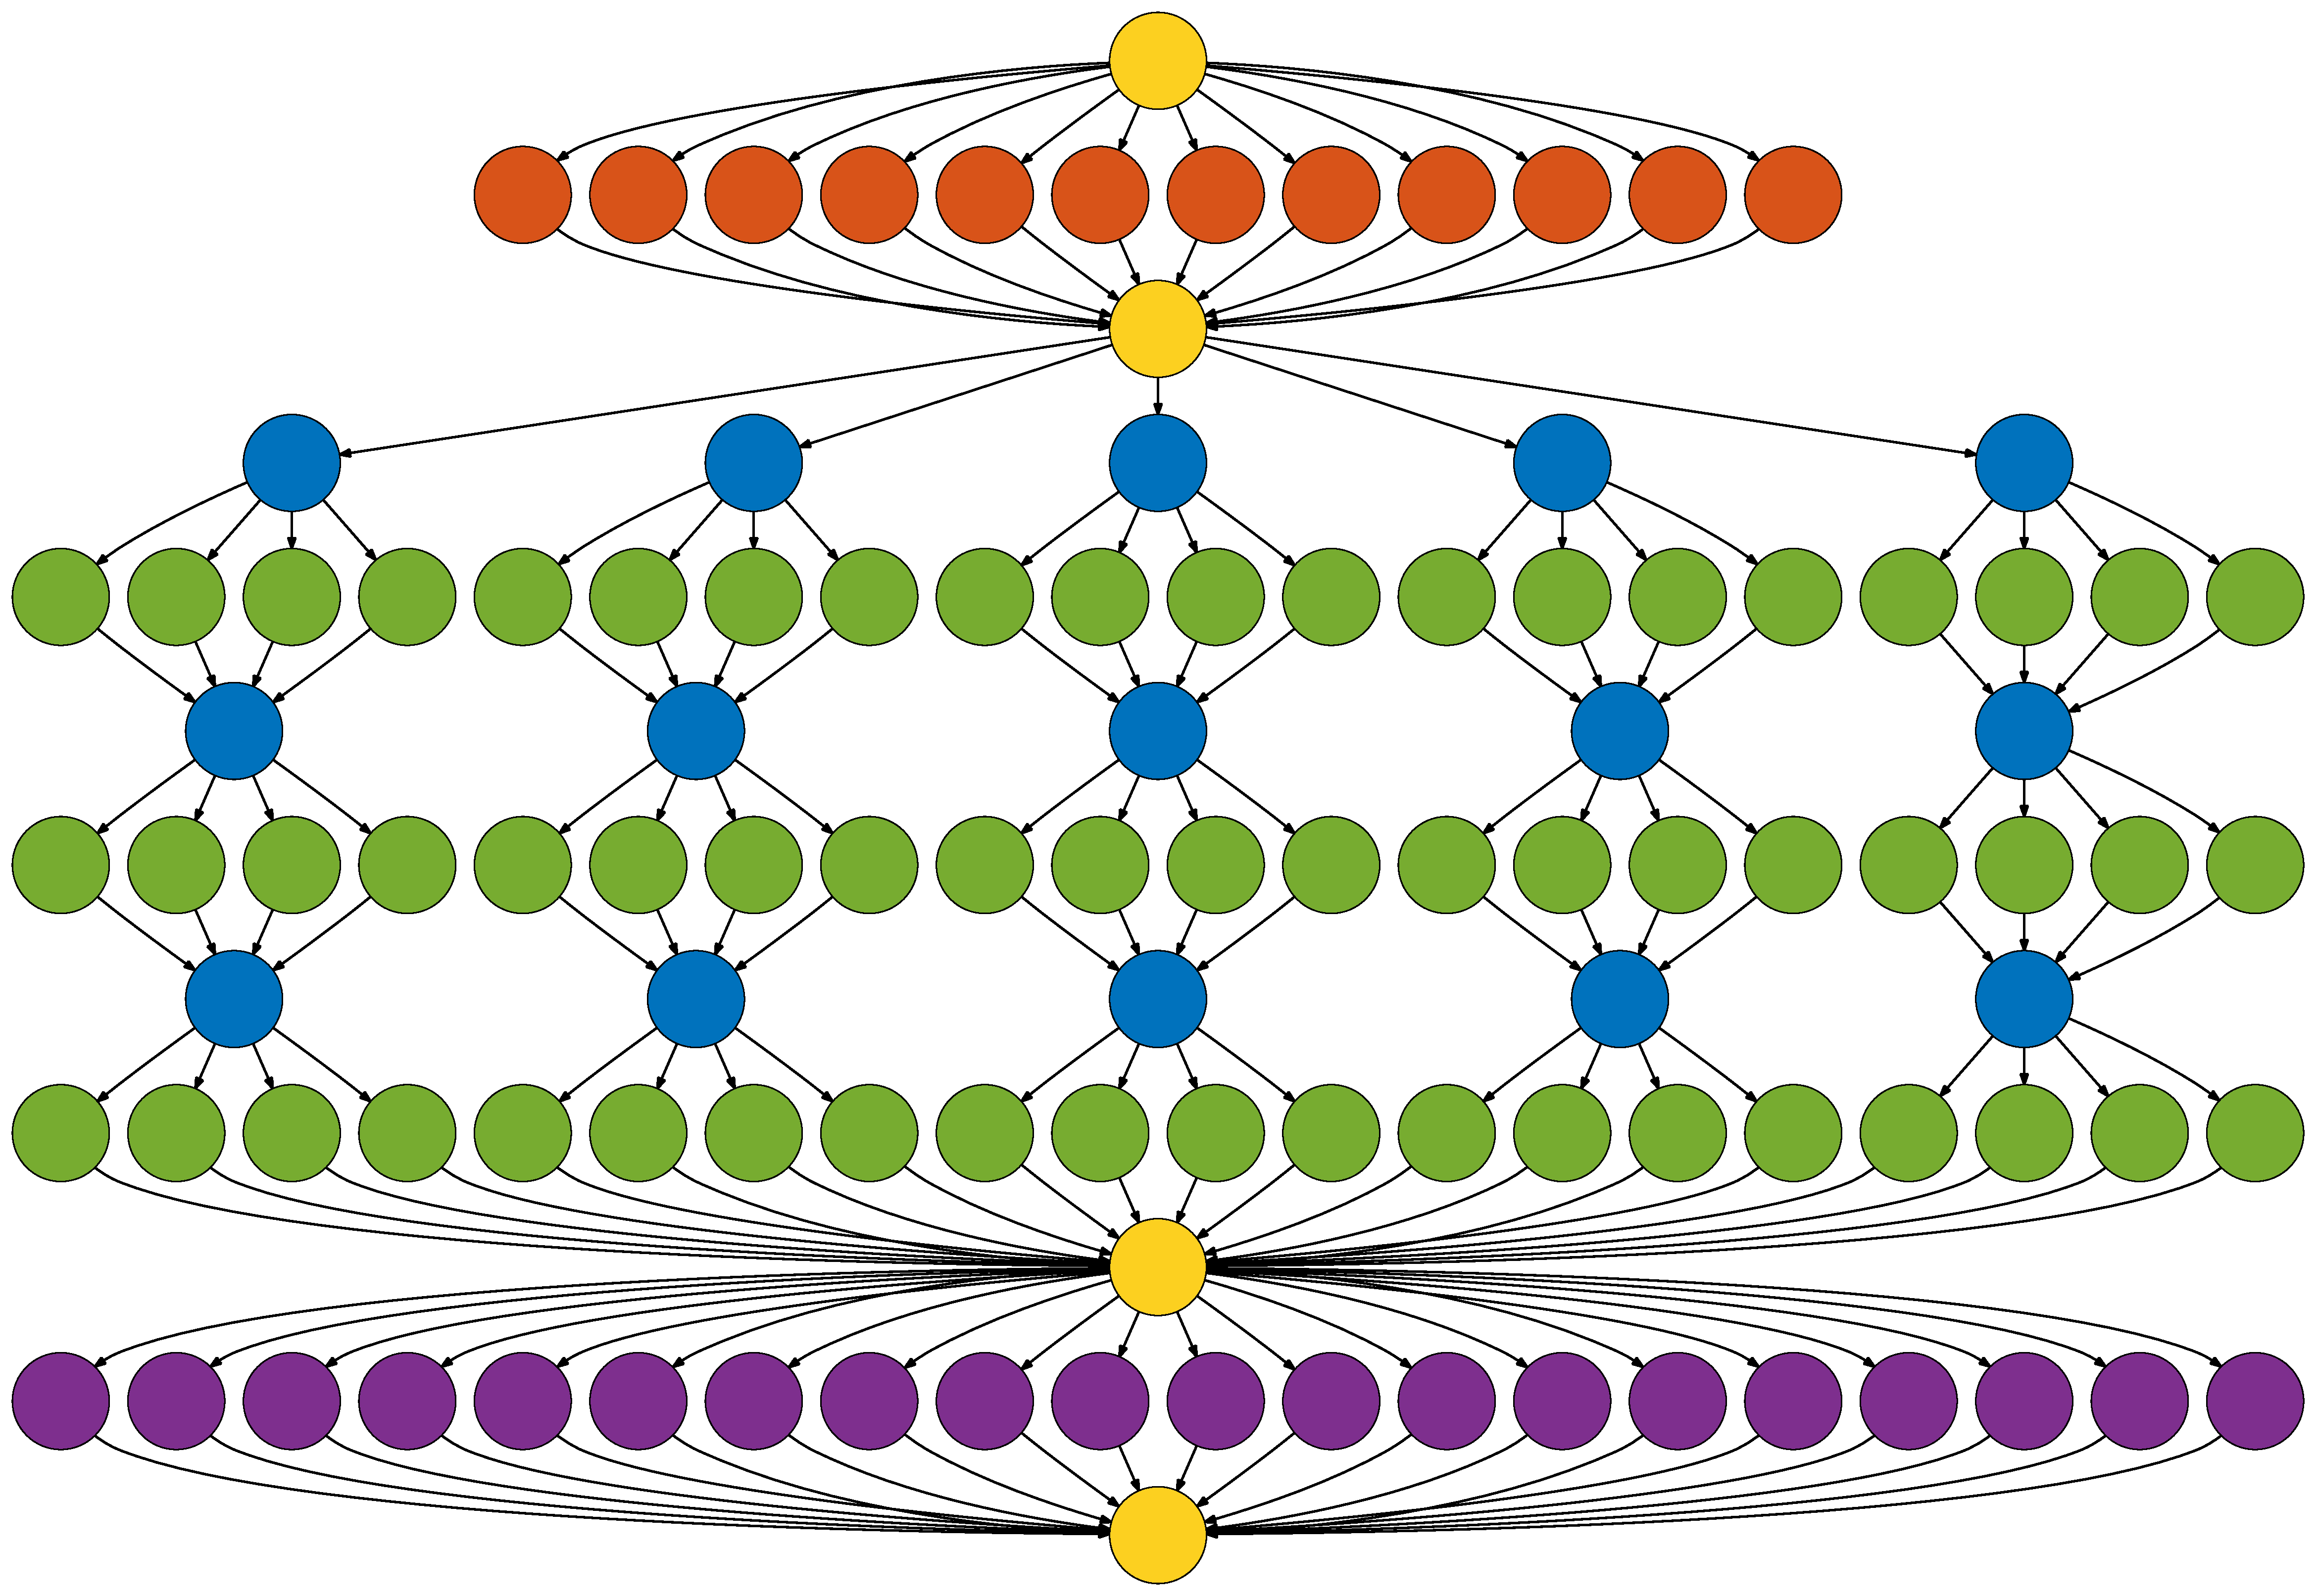
\includegraphics[width=0.95\columnwidth]{fig/deps}
  \end{center}
  \caption{Task dependencies of a convolutional layer.}
  \label{fig:task_deps}
\end{figure}


The main idea of the algorithm is to break up the computation of the
convolutional layer into tasks that operate on an independent chunk of
data.  We then create a task dependency graph and execute the tasks
using $N$ workers.  To increase cache locality the tasks are managed
using the work stealing scheduler, which means that each worker keeps
a list of local tasks as a stack (last task put on the stack will be
executed next)~\cite{reinders2007intel}.  If a local stack is empty,
only then a worker \emph{steals} and executes a task from other
worker's queue.

We have 5 types of task, each of which performs relatively simple
work.  A task dependency diagram is shown on
figure~\ref{fig:task_deps}.

The first type of tasks (yellow) have two purposes.  They serve as
synchronization points, and they deal with memory management.  They
allocate memory required for the next stage and free the memory that
is not needed any more.  The topmost yellow task allocates memory for
the FFT transforms of all the input images, as well as working memory
for each of the $N$ workers.

The second task type (red) performs a transform of a single image of
the input.  Note that performing FFTs of image require some extra
working memory, which was allocated for each worker in the dependent
yellow task.  The number of such tasks will equal to the product of
the batch size and the number of input feature-maps.

After computing all the FFTs transforms of all the input images, we
can free the memory used by the images (as we don't need that
information anymore).  This is done by the second from the top yellow
task.  This yellow task also allocates memory for FFTs of all the
output images.

The next two task types are blue -- performs the FFT transform of a
kernel, and green -- multiplies the FFT transform of the kernel with
the appropriate FFT transform of the input image and adds to the
appropriate sum.  The task dependency is designed such that there's
never two workers trying to access the same memory.  Notice that the
blue tasks form some sort of a grid.  The blue tasks in each column
operate on the same output feature map, and blue tasks in each row
operate on the same input feature map.  More specifically a blue task
in column $i$ and row $j$ represents performing the FFT of the kernel
$k_{i,j}$.  For each blue task there is a number of green tasks equal
to the batch size.

\subsection{GPU implementations}

\subsubsection{Direct convolution using CuDNN}

\subsubsection{FFT based algorithm}



%\begin{algorithm}
%  {\small
%  \begin{codebox}
%    \Procname{$\proc{Linear-index-map}(i,x_i,y_i,y_o)$}
%    \li $b \gets i / y_i$
%    \li $i \gets i - b \times y_i$
%    \li $r \gets b / x_i$
%    \li $b \gets b - r \times x_i$
%    \li \Return $(r \times y_i + i) \times y_o + b$
%  \end{codebox}
%  }%
%
%  \caption{Index mapping between two 3D matrices.  The input matrix
%  had dimensions $b \times x_i \times y_i$, and the output $b \times
%  y_i \times y_o$} \label{alg:index_map}
%\end{algorithm}


\section{Algorithms for the max fragment pooling layers}

\subsection{CPU algorithm}
\subsection{GPU algorithm}

\section{Sliding window inference}

We describe how sliding window works.  Reference ZNN paper and other
papers.  Explain a bit about our implementation.

Also explain how sparse inference works, as we will use that on the
GPU -- only available implementation in 3D.

Explain how the FLOPs per output voxels are computed.

Figures -- chars of FLOPS vs Memory for different algorithms.

Note -- The tables in the previous section are correct even when
rarefied kernels are used, the only thing that changes is the size of
the output image that now equals $n' = n - (k-1)*r$, where $r$ is the
sparseness of the kernel.



\begin{figure}
  \begin{center}
  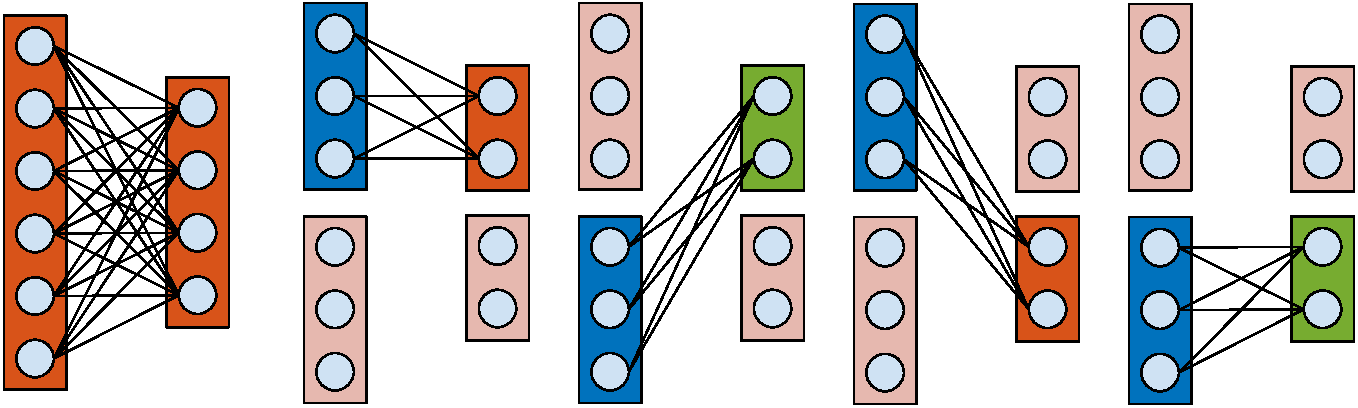
\includegraphics[width=0.95\columnwidth]{fig/gpuram.pdf}
  \end{center}
  \caption{Partial loading of data to the device.}
  \label{fig:partial_exec}
\end{figure}

Pooling layers use CUDNN.

Direct convolutional layers also use CUDNN.  If possible they use the
pre--computed gemm which requires workspace memory.  The cases when
this is possible is not well documented so we experimentally determine
whether we can use it.

FFT convolutional layers are implemented in the following way.  For
each layer we do the following.  We transform all the inputs first.
We break up the input into largest possible chunks that can be
transformed with CUFFTPLANN.  Once we have all the input transforms
(of all the images and bathes) we compute one output image at the
time.  For $i$-th output image we compute FFTs of all the relevant
kernels, then for each batch we compute the point-wise product of the
FFTs of the input images and the FFTs of the kernels.  We accumulate
the result into a single image using a matrix vector product CUBLAS
where the vector has all ones.  We repeat the process for every $i$-th
output of every batch, as we want to re-use the FFTs of the computed
kernels.

Finally we compute the inverse transform of the output images, scale
them appropriately, add the bias and apply the transfer function.

We carefully design the steps in order to minimize the extra memory
utilization.


\section{Experiments}

\subsection{Purely convolutional networks}
\subsection{Max-pooling convolutional networks}


\begin{figure*}[h!t]
  \centering
  \subfloat[]{\protect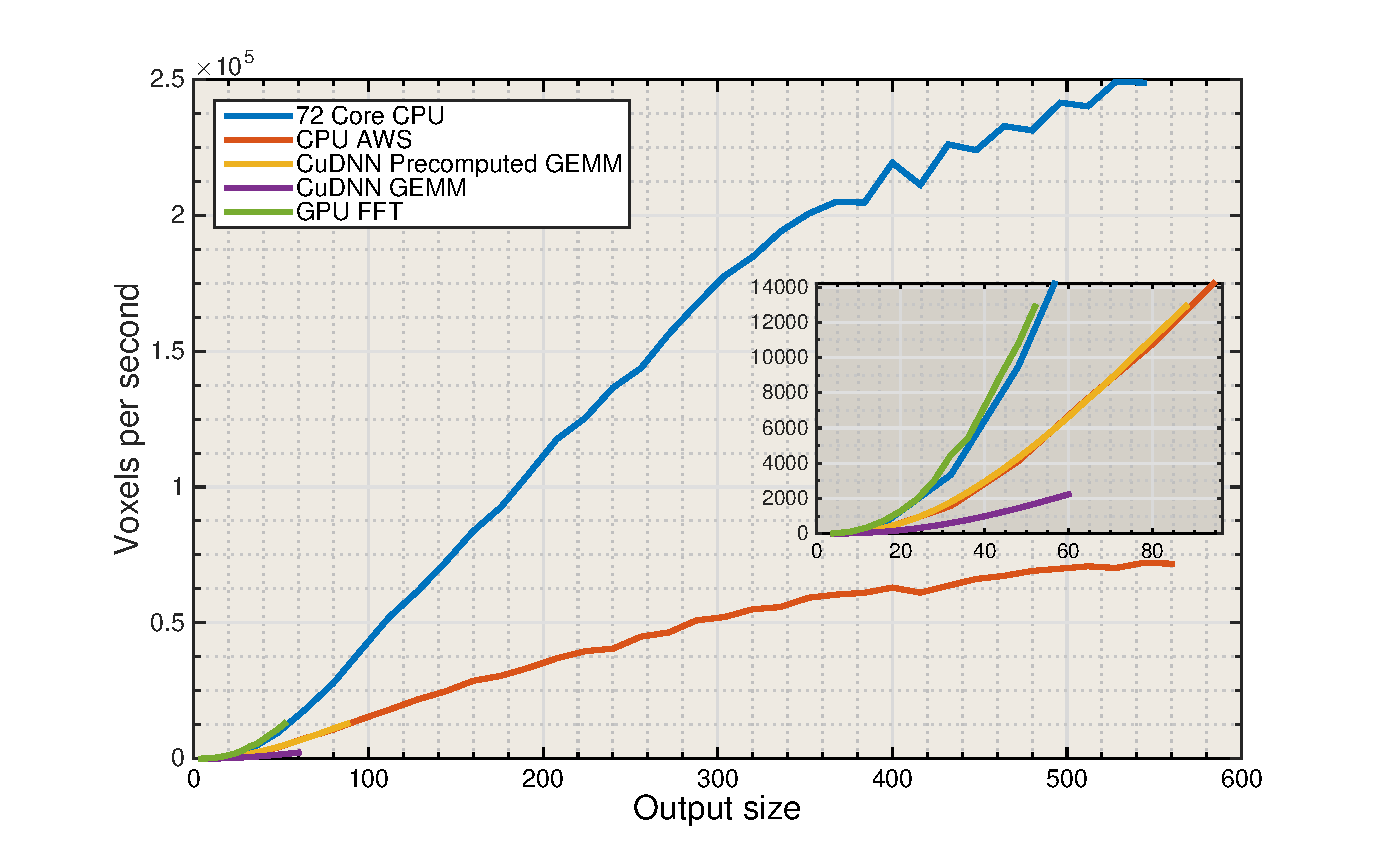
\includegraphics[width=0.44\textwidth]
    {fig/m96.eps}}
  \subfloat[]{\protect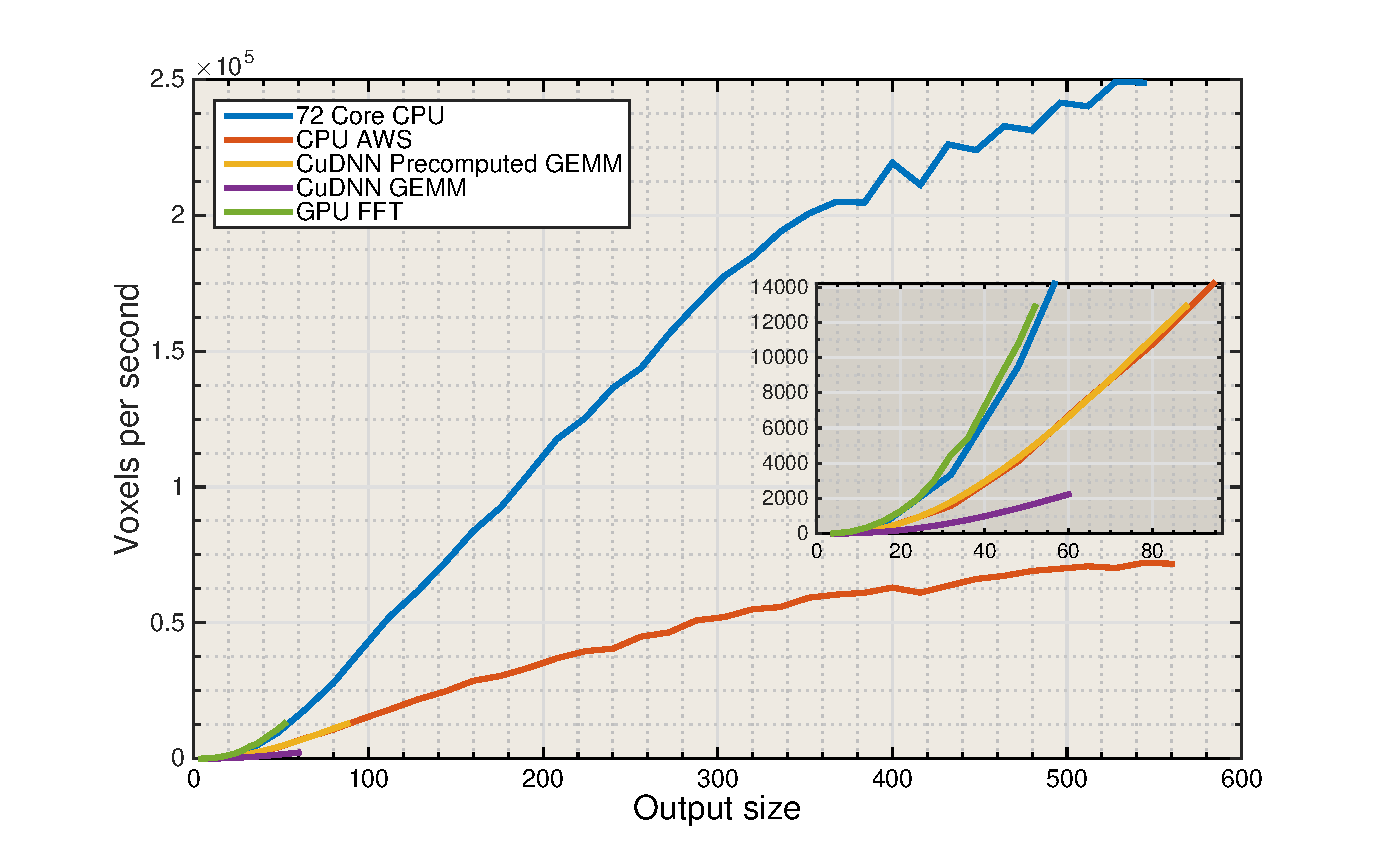
\includegraphics[width=0.44\textwidth]
    {fig/m96.eps}}
    \\
  \subfloat[]{\protect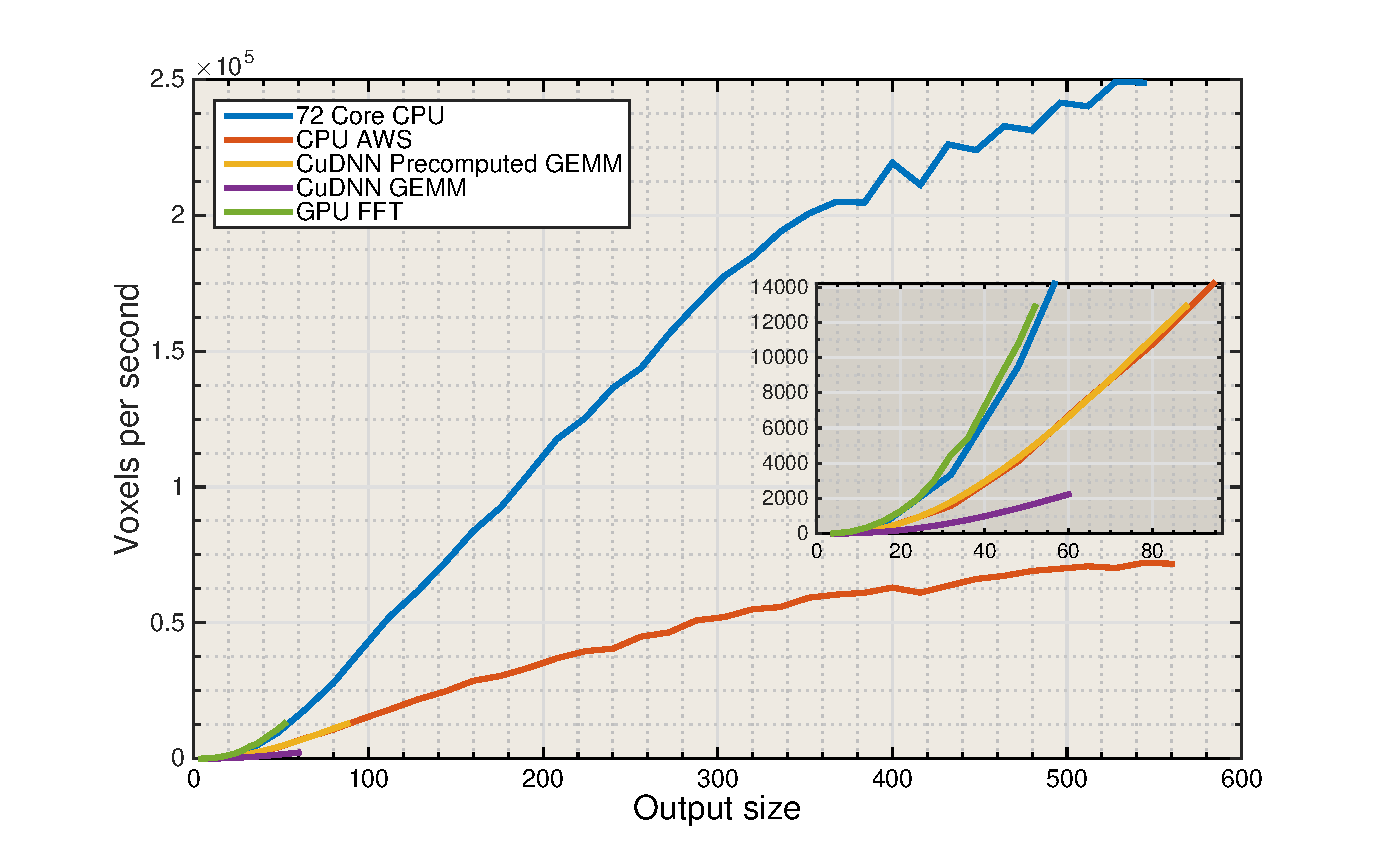
\includegraphics[width=0.44\textwidth]
    {fig/m96.eps}}
  \subfloat[]{\protect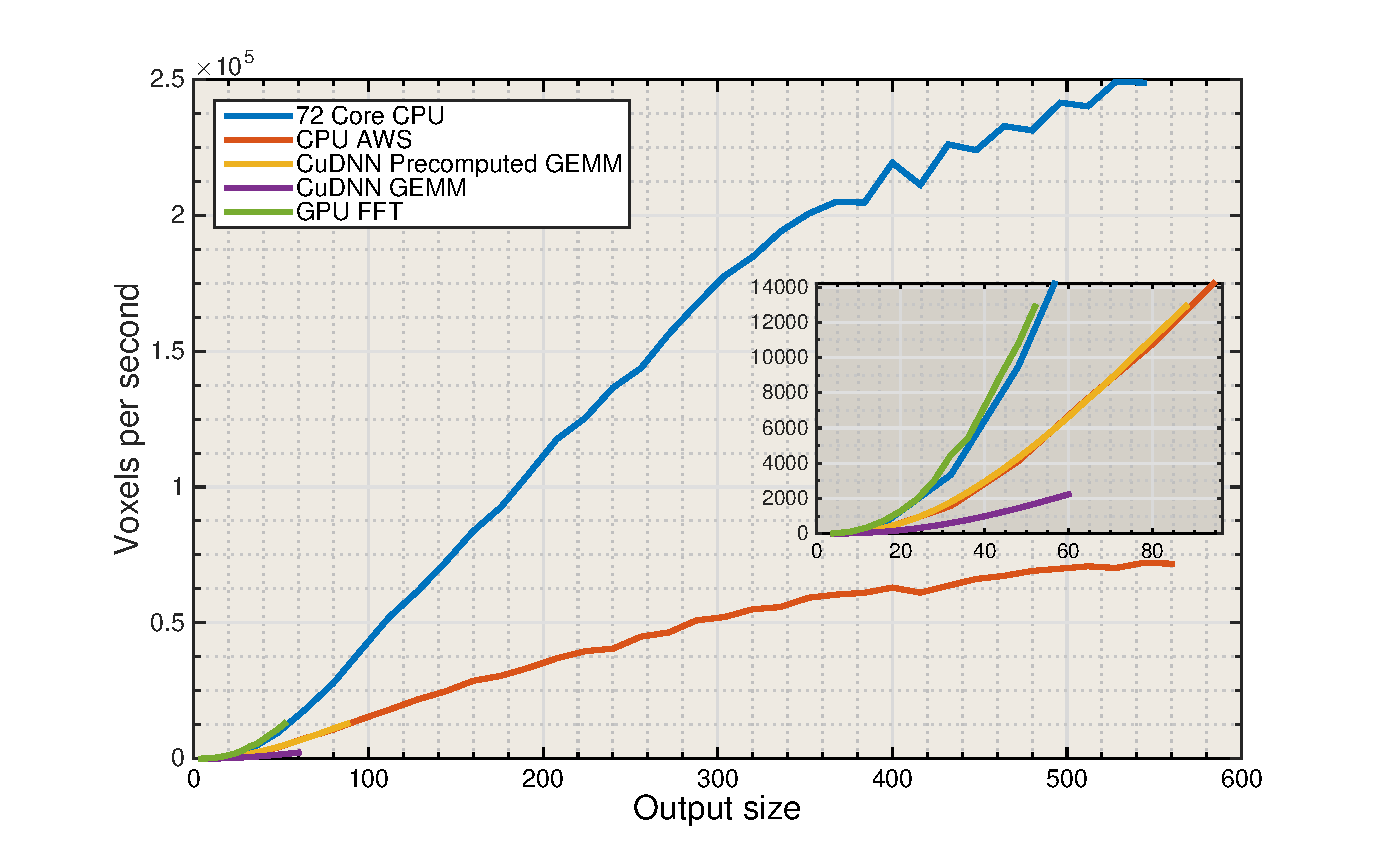
\includegraphics[width=0.44\textwidth]
    {fig/m96.eps}}

  \caption{Throughput vs output patch size for pooling networks
  }
  \label{fig:2dspeedups_threads}
\end{figure*}


\begin{figure*}[h!t]
  \centering
  \subfloat[]{\protect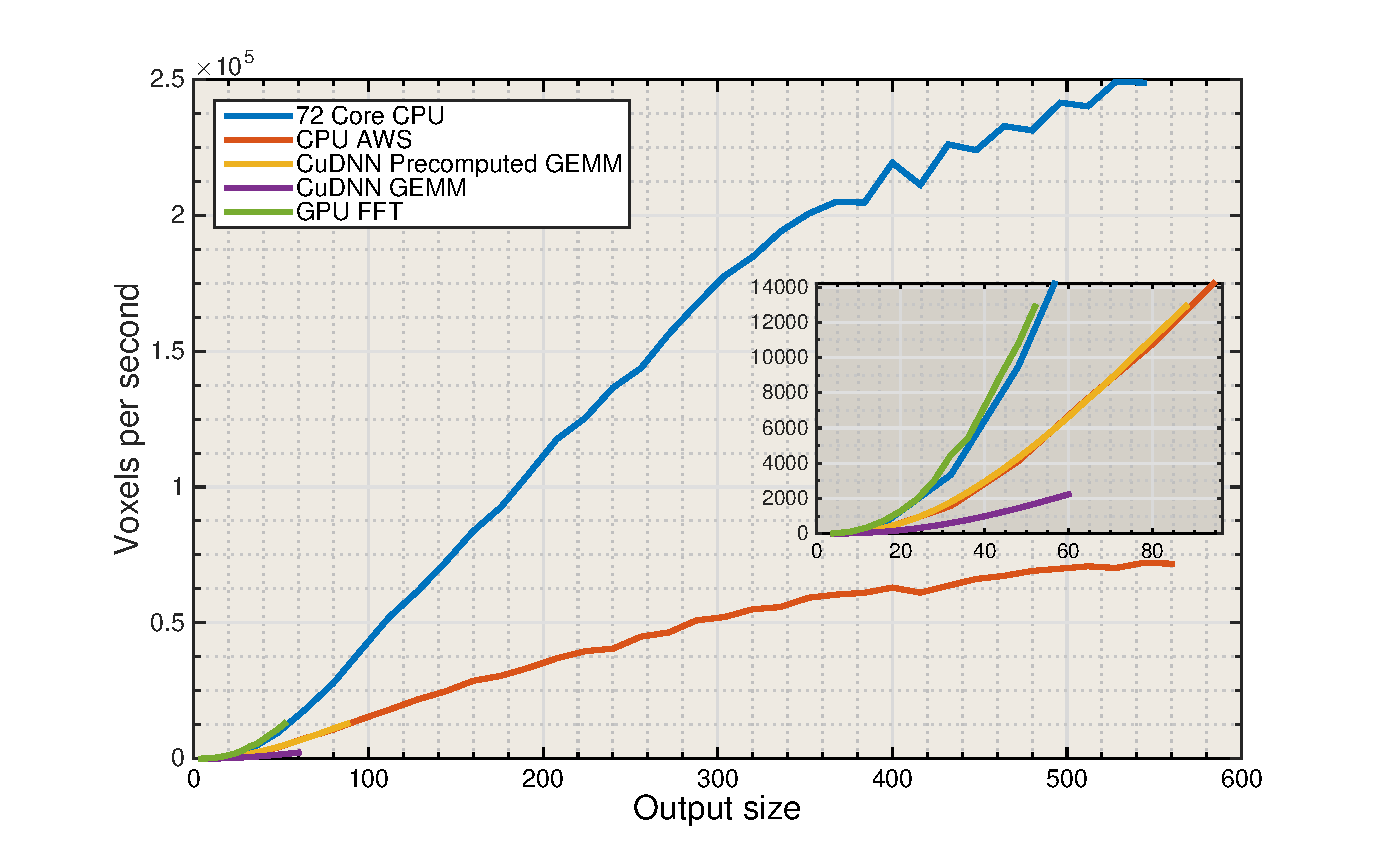
\includegraphics[width=0.44\textwidth]
    {fig/m96.eps}}
  \subfloat[]{\protect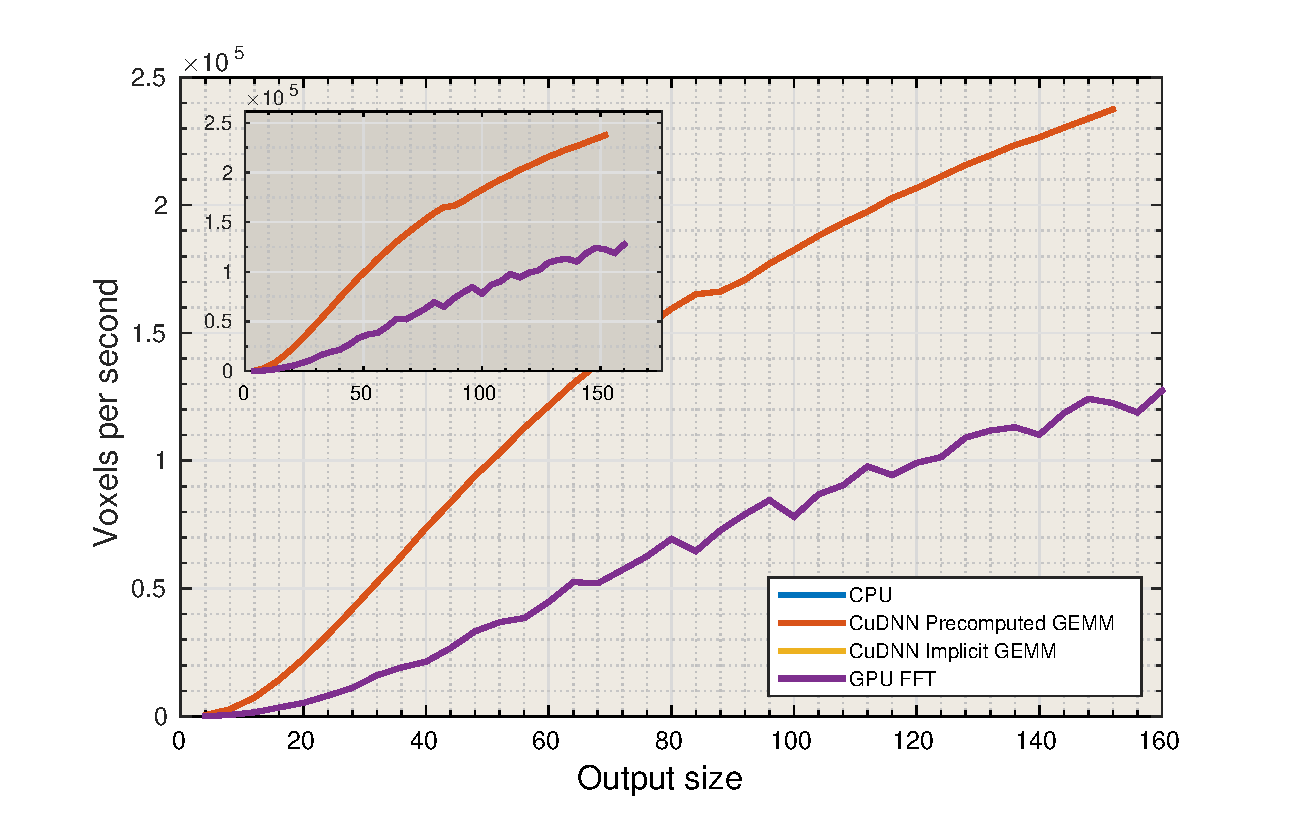
\includegraphics[width=0.44\textwidth]
    {fig/m56.eps}}
    \\
  \subfloat[]{\protect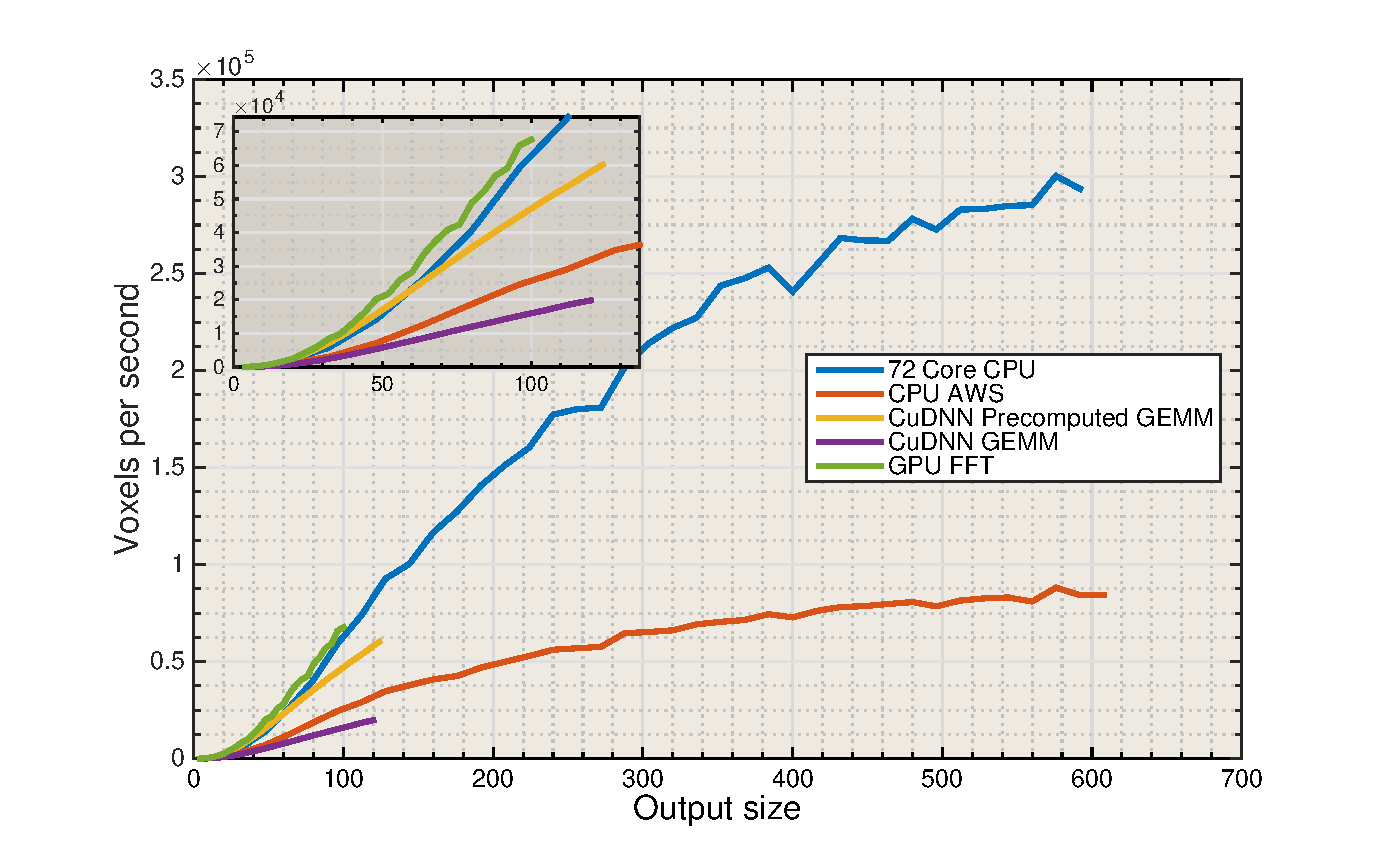
\includegraphics[width=0.44\textwidth]
    {fig/m76.eps}}
  \subfloat[]{\protect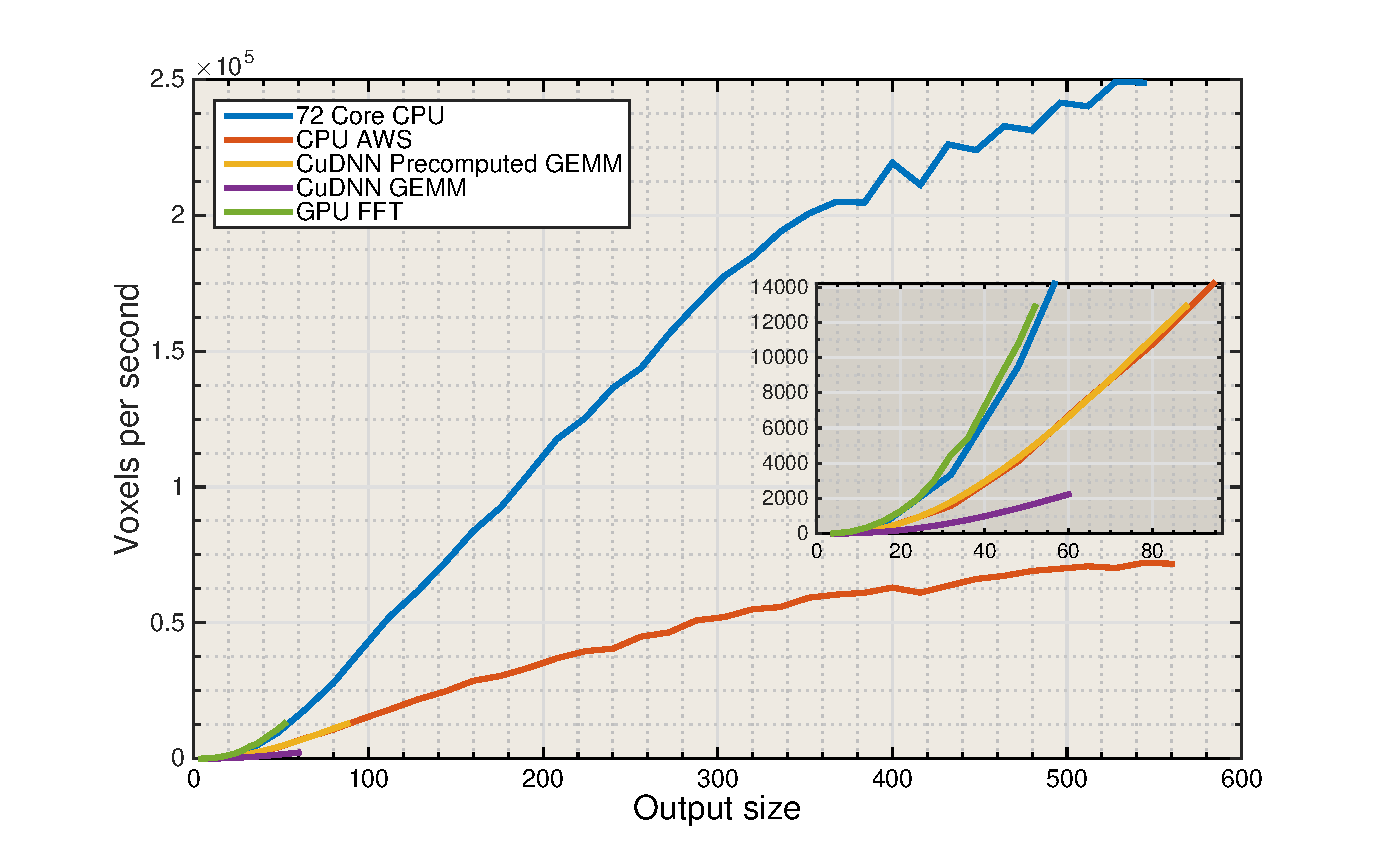
\includegraphics[width=0.44\textwidth]
    {fig/m96.eps}}

  \caption{Throughput vs output patch size for pooling networks
  }
  \label{fig:2dspeedups_threads}
\end{figure*}


%%%%%%%%%%%%%%%%%%%%%%%%%%%%%%%%%%%%%%%%%%%%%%%%%%%%%%%%%%%%%%%%%%%%%%%
%%%%%%%%%%%%%%%%%%%%%%%%%%%%%%%%%%%%%%%%%%%%%%%%%%%%%%%%%%%%%%%%%%%%%%%
%%
%% REFERENCES
%%
%%%%%%%%%%%%%%%%%%%%%%%%%%%%%%%%%%%%%%%%%%%%%%%%%%%%%%%%%%%%%%%%%%%%%%%
%%%%%%%%%%%%%%%%%%%%%%%%%%%%%%%%%%%%%%%%%%%%%%%%%%%%%%%%%%%%%%%%%%%%%%%


{\small
\bibliographystyle{IEEEtran}
\bibliography{IEEEabrv,./ref/bib}
}

\end{document}

%% ZNN - A Fast and Furious Technique for Training ConvNets on
%% Multi-Core and Many-Core Shared Memory Machines

%% C = 5 (or 2.5) should be mentioned somewhere?
